\section{Particle model}
\label{sec:physical}
\label{sec:model}
\label{sec:thermo}

This section states the particle model that the rest of the paper
exercises: the phase regimes of one particle, the balances in each region,
the conditions that close the moving front and the properties that enter
them. Readers mainly interested in the process results can read
Section~\ref{sec:physical:regimes} and then continue with
Section~\ref{sec:validation}.

\subsection{Particle geometry, inventories and phase regimes}
\label{sec:physical:regimes}
\label{sec:physical:threshold}
\label{sec:physical:inversion}
\label{sec:physical:lewis}

The model follows one particle through three regimes, defined by where
liquid hexane remains. Hexane is stored as external free hexane, hexane in a
liquid-hexane core, retained hexane and pore gas.
External free hexane wets the surface in regime A. Its depletion allows the
liquid-hexane core to recede in regime B, leaving a dry shell. Throughout
this paper, \emph{dry shell} means depleted of free liquid hexane, not free
of water or retained hexane. Regime C begins when the liquid-hexane core
disappears. Steam can form an external water film, from which
\emph{liquid-water imbibition} transfers water into the particle's retained-water
inventory. Retained water includes effective matrix and interstitial
retention; it does not imply that all water is molecularly bound.

We approximate the particle by a porous sphere of fixed radius $\Rp$.
This geometry resolves radial heat and mass transport with one length
scale, as in the particle descriptions of \citet{faner2019kinetics} and
\citet{cardarelli2002modeling}. Actual meal particles are irregular;
the radius selected for each experiment is therefore stated with its
source and interpretation. Fixed radius and porosity separate transport
from swelling and shrinkage, for which no constitutive laws are supplied here.
The particle's total n-hexane loading $\Xh$ (every loading here in
\si{\kilogram} per \si{\kilogram} of dry, water- and solvent-free meal)
is compared with two thermodynamic reference loadings at the particle's
temperature. The first is the critical loading $\Xc(T)$, at which mobile
liquid stops reaching the outer surface; it is set on the transition loading
\citet{faner2019kinetics} measured (Table~\ref{tab:parameters}). The second is the equilibrium loading
$\Xe^{*}(T,P)$, at which no condensed hexane remains. The star denotes
evaluation at the pressure-feasible saturated activity $a^{*}$ of
Eq.~\eqref{eq:aceiling}. In regime~A, while external free hexane remains,
bulk liquid wets the outer surface at unit hexane activity and the resistance
is external. In regime~B ($0<\front<\Rp$), liquid is present only behind a
receding interface, and removal is limited by the heat reaching that interface
through a growing dry shell. In
regime~C, no liquid-hexane core remains: $\front=0$. Retained material and
pore gas continue to obey the same local component and energy balances.
Core extinction is a geometric conservation event; a particle-mean loading
is not used to prescribe it. The saturated equilibrium loading is a
thermodynamic reference rather than a uniform-particle transition rule
(Figure~\ref{fig:schematic}).

\begin{figure}[htbp]
\centering
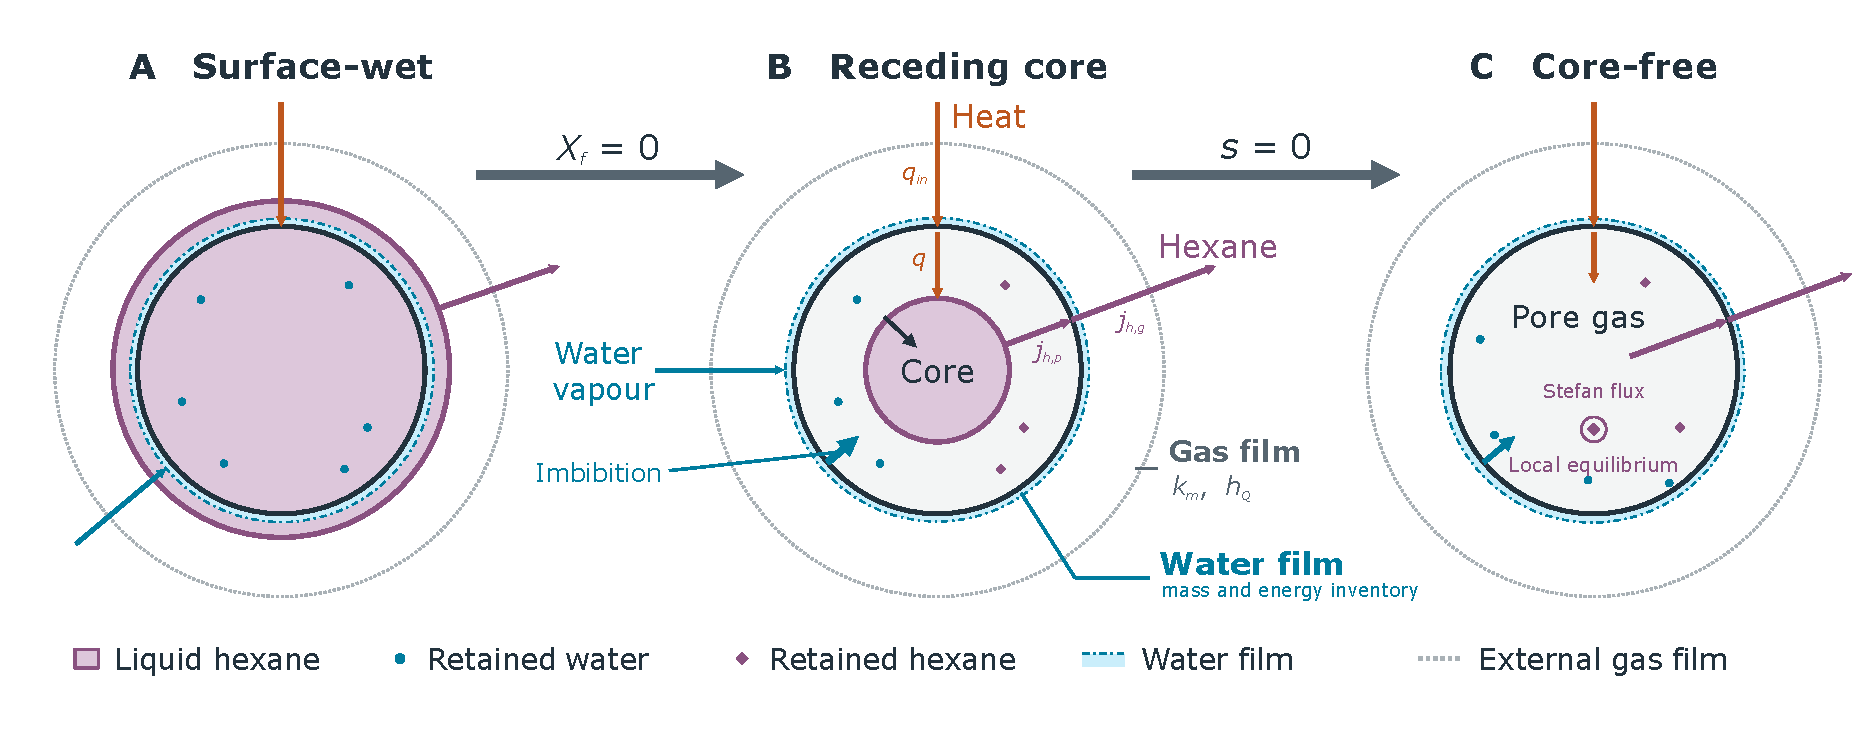
\includegraphics[width=\textwidth]{figures/fig_particle_model.pdf}
\caption{Particle regimes and transport pathways.}
\label{fig:schematic}
\end{figure}

Figure~\ref{fig:schematic} follows external free-hexane depletion
($\Xf=0$) and subsequent core disappearance ($\front=0$).
Purple represents hexane and blue represents water; orange arrows show
incoming heat. The dashed blue band is the optional external water film,
through which hexane can escape in the proposed closure. Liquid-water
imbibition operates in the dry shell connected to that film, with no
additional liquid-water flux into the liquid-hexane core. Dots and diamonds
represent retained water and retained hexane, respectively. Geometry and
film thickness are schematic. Fluxes are outward-positive: $j$ is
mass-based and $N$ molar, with $h_k^{\mathrm{mass}}=\bar h_k/M_k$;
subscripts p and g identify the particle and gas sides of the surface.

The particle model is written so that it can later be coupled to a tray
model. For prescribed gas and heat-transfer conditions, the particle balances return
outward-positive surface fluxes $j_{\mathrm{w}}(\Rp)$,
$j_{\mathrm{h}}(\Rp)$ and $\JE(\Rp)$ on one caloric datum. These are
responses to the evolving interior, rather than imposed drying rates. For
particle classes $c$ with total exposed areas $A_{\mathrm{ex},c}$, the rates
delivered to a future tray gas balance would be
$\sum_c A_{\mathrm{ex},c}j_{k,c}(R_{p,c})$ for component $k$ and
$\sum_c A_{\mathrm{ex},c}J_{E,c}(R_{p,c})$ for total energy. Condensation has a
negative water rate; each gas source has an equal and opposite entry in
the particle balance. The tray would return its updated gas state to the particles.
In this paper, the gas and bed conditions along the equipment trays are
prescribed instead. This separates the particle response from countercurrent
gas mixing and tray residence, which is useful for testing the particle equations before
coupling them to DT design calculations; steam consumption itself requires
those equipment balances \citep{kemper2013solvent}.

The equilibrium boundary is evaluated at the \emph{pressure-feasible} hexane
activity
\begin{equation}
a^{*}(T,P) \;=\; \min\!\left(1,\;P/P_{\mathrm{sat}}^{\mathrm{h}}(T)\right),
\label{eq:aceiling}
\end{equation}
with $P$ the total pressure and $P_{\mathrm{sat}}^{\mathrm{h}}$ the n-hexane
vapour pressure, both in pascals. Equation~\eqref{eq:aceiling} is an
ideal-mixture diagnostic. The pore and interface equilibrium used in the
calculations uses binary-virial gas fugacities and the pure-liquid equation-of-state
fugacities on the same pressure and caloric datum. It does not omit those
corrections when locating phase boundaries. Above the solvent's
boiling point at the bed pressure, an equilibrium loading taken at unit
activity is overstated. Evaluated with
\eqref{eq:aceiling}, the two boundaries stay one to two orders of magnitude
apart and separate further as the temperature rises; the paper uses only that
\emph{ordering} (Sec.~\ref*{S-sup:regime}).

The A--B transition occurs when the external free-hexane inventory
$\Xf$ is exhausted. While $\Xf>0$, liquid wets the surface and the front stays at
$\front=\Rp$; once $\Xf=0$, it may recede and leave a dry shell. This
sequential-drainage condition is stated in Eq.~\eqref{eq:complementarity}.
The reference critical loading of
\SI{0.20}{\kilogram\per\kilogram} measured by
\citet{faner2019kinetics} sets the effective critical-volume capacity
at the reference liquid density, 615 kg/m$^3$. At the particle's actual
temperature, $\Xc(T)=\kappa_v\varepsilon_{\mathrm g}
\rho_{\mathrm{h,l}}(T,P)/\Cdm$, with $\kappa_v=2.675$ fixed by that
reference capacity. The liquid density comes from the same equation of
state used in the component and energy balances. The depletion loading
therefore has a prescribed temperature dependence, while the time at which
it is reached follows from the regime-A inventory balance under the
prescribed gas and heat history. The component and energy jumps then determine the recession speed
and the dry-side hexane flux at the front. The shell balances and surface
conditions determine the corresponding particle-surface exchanges. In the
discrete model the front first departs over
an accepted time step, giving a finite shell thickness without assigning the
shell the width of one radial cell (Sec.~\ref*{S-sup:item27}). The A--B
boundary is thus a surface-state constraint, with no fitted time or drying-rate
selector. The stationary binary regime-C closure starts after the liquid-hexane core
has vanished. In a calculation, the crossing \emph{loading} therefore
reproduces a supplied value; the crossing \emph{time} is the tested
prediction, conditional on the external history
(Section~\ref{sec:validation:faner}).

Heat must first cross the gas-side resistance and then the dry shell to
reach the receding front. In the reported scale comparison, the external
thermal resistance dominates until the core radius falls to about
$0.28\Rp$; the dry-shell resistance dominates later
(Sec.~\ref*{S-sup:closures}). The present total-vapour closure adds no
pressure-driven transport resistance, so front recession is heat-limited.
This distinction matters when interpreting falling-rate data: the 2019
Faner records support a heat-limited description, whereas the older
Faner records and the mechanism of \citet{cardarelli2002modeling} support
a diffusion-limited description. The separate scalar Fickian comparison
in Eq.~(\ref*{S-eq:ficklimit}) represents the latter; it does not replace
the shared particle law in either experiment
(Sec.~\ref*{S-sup:tworegimes}).

Temperature and composition also vary over different radial scales. The
dry-shell Lewis number of $223.25$ requires their profiles to be
reconstructed separately near the moving front
\citep{crank1956diffusion,perre2023stateoftheart}.

\subsection{Local balances and region closures}
\label{sec:model:geometry}
\label{sec:model:local}
\label{sec:model:wet}
\label{sec:model:dry}

Inside each region the model is a set of conservation laws with no source
terms, closed differently in the liquid-hexane core and in the dry shell. The sphere
holds two conserved mobile components, water and n-hexane, and an immobile
composite dry meal of local density $\Cdm$ with a residual-oil mass
fraction $\wo$. A sharp interface at radius $r=\front(t)$, with $t$ the time,
separates a liquid-hexane core ($\mathrm{w}$) from a dry shell ($\mathrm{d}$); the
region label $\alpha$ takes either value. Radial fluxes are positive
outward, and recession means $\dot{\front} < 0$. The total radial energy flux is
defined once, on both sides, as
$\JE^{\alpha} = q^{\alpha} + \sum_{k} \bar{h}_{k}^{\alpha} j_{k}^{\alpha}$,
with $q$ the conductive heat flux, $j_{k}$ the radial flux of component $k$
and $\bar{h}_{k}$ the partial molar enthalpy on the common datum of
Section~\ref{sec:thermo:datum}. In each smooth region
\begin{align}
\frac{\partial C_{k}^{\alpha}}{\partial t}
 + \frac{1}{r^{2}}\frac{\partial}{\partial r}\!\left(r^{2} j_{k}^{\alpha}\right)
 &= 0, \qquad k \in \{\mathrm{w},\mathrm{h}\},
\label{eq:localcomp}\\[2pt]
\frac{\partial u^{\alpha}}{\partial t}
 + \frac{1}{r^{2}}\frac{\partial}{\partial r}\!\left(r^{2} \JE^{\alpha}\right)
 &= 0,
\qquad j_{\mathrm{dm}} = 0, \qquad j_{L_{\mathrm{o}}} = 0 ,
\label{eq:localenergy}
\end{align}
with $C_{k}$ the total local concentration of component $k$ over all of its
phases, $u$ the total local internal energy density, and $j_{\mathrm{dm}}$
and $j_{L_{\mathrm{o}}}$ the fluxes of the immobile dry meal and residual oil.
Retention,
evaporation and condensation redistribute a component between local phases and
are therefore \emph{not} sources in \eqref{eq:localcomp}: no phase-change term
appears in the smooth-region equations (Sec.~\ref*{S-sup:ale}).

Two statements close the liquid-hexane core. First, no relative n-hexane flux is carried inside
the mobile-liquid region: at activation, every material shell stores the
historical label $\Xhwa = \Xc(\theta_{a})$, the critical loading at its
temperature at activation $\theta_{a}$, and thereafter
\begin{equation}
\frac{\mathrm{D}_{s}}{\mathrm{D}t}\!\left(\Cdm\,\Xhwa\right) = 0
\label{eq:shellconserved}
\end{equation}
following the solid. Thus $\Xhwa$ is the apparent mobile-liquid hexane
loading of the liquid-hexane core, stored at activation and distinct both from the
particle's total loading $\Xh$ and from the retained hexane of the dry
shell. The core is liquid-filled, the hexane activity is unity,
and the non-negativity of the mobile liquid is an admissibility condition, not
a clipped quantity. Second, the core is resolved, not lumped, with specific energy
per kilogram of dry meal
\begin{equation}
e_{\mathrm{w}} \;=\; h_{\mathrm{dm}}(T,\wo)
 \;+\; \Xw\, h_{\mathrm{w,l}}(T,P)
 \;+\; \Xhwa\, u_{\mathrm{h,l}}(T,P)
 \;-\; \Bh(\ah{=}1,T,\wo),
\label{eq:wetenergy}
\end{equation}
with $h_{\mathrm{dm}}$ the specific enthalpy of the dry meal, $\Xw$ the total
water loading, and $h_{\mathrm{w,l}}$ and $u_{\mathrm{h,l}}$ the specific
enthalpy of liquid water and the specific internal energy of liquid n-hexane,
both in \si{\joule\per\kilogram}. Retained and mobile hexane are not
carried separately in this energy, so the binding
potential $\Bh$ is counted once and the repartition between them is source-free.

The dry shell stores each component in two forms, pore gas and a retained
contribution, with distinct storage terms and distinct thermodynamics; no
retained-only symbol includes pore gas. Transport
consists of one thermodynamic-force pore flux, one retained-matrix water flux and one
algebraic total flux,
\begin{align}
J_{\mathrm{w}} \;=\; -J_{\mathrm{h}}
 &\;=\; -\Lwh\,\nabla_{\mathrm{comp}}\!\left[\frac{\mu_{\mathrm{w}}-\mu_{\mathrm{h}}}{RT}\right],
\label{eq:binaryflux}\\[2pt]
N_{\mathrm{w,ret}}
 &\;=\; -\Lwr\,\nabla_{\mathrm{comp}}\!\left[\frac{\mu_{\mathrm{w,ret}}}{RT}\right],
\qquad
N_{i}^{\mathrm{g}} = y_{i}\Nt + J_{i} ,
\label{eq:retflux}
\end{align}
with $\mu_{\mathrm{w}}$ and $\mu_{\mathrm{h}}$ the pore-gas chemical potentials
of water and n-hexane and $\mu_{\mathrm{w,ret}}$ that of retained water
(\si{\joule\per\mole}), $R$ the gas constant, $\Lwh$ and $\Lwr$ the pore and
retained-matrix mobilities (\si{\mole\per\meter\per\second}), $y_{i}$ the
pore-gas mole fraction of component $i$, and the fluxes $J_{i}$,
$N_{\mathrm{w,ret}}$, $N_{i}^{\mathrm{g}}$ and $\Nt$ molar
(\si{\mole\per\meter\squared\per\second}). The total (Stefan) flux $\Nt$ is recovered algebraically from the summed
continuity equations rather than fitted. It rests on an Onsager mobility whose
degeneracy vanishes exactly at either purity and needs no composition floor
\citep{krishna1997maxwell}. The shell energy flux carries each stream exactly
once, with no latent, binding, pressure-volume or Stefan-energy correction on
top (Sec.~\ref*{S-sup:stefanrecovery}). We retain composition-driven mass transport and conductive heat transport,
and neglect independent Soret terms because no thermal-diffusion
coefficients for this meal are supplied. This is a constitutive approximation;
it does not show that thermal diffusion is negligible. Here $\nabla_{\mathrm{comp}}$ denotes the composition part of the
fixed-$(T,P)$ chemical force, not the full gradient of a temperature-dependent
standard chemical potential. At ordinary faces, the isothermal
composition secant is evaluated at a common face temperature. The moving-interface
reconstruction integrates that composition derivative along the actual
linear temperature/composition path,
\begin{equation}
G_{\mathrm{comp}}(\Xi)=\frac{1}{d}\int_0^1
\left.\frac{\partial\Xi}{\partial y_{\mathrm h}}\right|_{T(\lambda),P}
\frac{\dd y_{\mathrm h}}{\dd\lambda}\,\dd\lambda,
\qquad \Xi=\ln(f_{\mathrm w}/f_{\mathrm h})
\ \hbox{or}\ \ln(f_{\mathrm w}/f_{\mathrm{ref}}).
\end{equation}
Here $d$ is the face separation and $f_i$ is the equation-of-state fugacity.
Energy transport remains non-isothermal and includes component enthalpies.
This is the declared nominal transport approximation in both prescribed-bath experiments.
The pressure variation omitted by
taking $\Nt$ from continuity is estimated from Darcy's law across the dry
shell,
\begin{equation}
\Delta P \;\approx\; \frac{\Nt\, R T}{P}\,\frac{\mu_{g}}{B}\,(\Rp-\front),
\label{eq:darcy}
\end{equation}
with $\mu_{g}$ the pore-gas viscosity and $B$ the Darcy permeability.
For an illustrative vapour-flux bound, take
$|\Nt|=\SI{0.5}{\mole\per\square\metre\per\second}$; this is a supplied
sensitivity scale, not the measured or calculated mean flux of the new DT
history. With this flux bound,
$\mu_{g}=10^{-5}\,\si{\pascal\second}$, $T$ at the heteroazeotrope and a
shell \SI{1}{\milli\metre} thick, the estimate gives $\Delta P$ of about
\SI{0.15}{\kilo\pascal}, \SI{1.5}{\kilo\pascal} and \SI{15}{\kilo\pascal}
at $B=10^{-12}$, $10^{-13}$ and $10^{-14}\,\si{\square\metre}$. A capillary
bundle $B=\varepsilon_{g} r_{\mathrm{pore}}^{2}/(8\tau)$ at the particle
porosity $0.14$ and a tortuosity of three is about
$10^{-13}\,\si{\square\metre}$ for a \SI{5}{\micro\metre} pore
($\Delta P$ about \SI{1}{\kilo\pascal} on the same bound) and about
$6\times 10^{-15}\,\si{\square\metre}$ for a \SI{1}{\micro\metre} pore
($\Delta P$ about \SI{25}{\kilo\pascal}). Below about
$10^{-15}\,\si{\square\metre}$ the estimate exceeds the bed pressure.
The isobaric closure therefore assumes that the vapour crosses a
connected pore space of several micrometers. It does not apply to a path
confined to sub-micrometer pores, and no measured permeability
of this meal is supplied here.
These fluxes do not reduce to a scalar Fick law for n-hexane.
Summing \eqref{eq:retflux} over the two components gives
$N_{\mathrm{w}}^{\mathrm{g}} + N_{\mathrm{h}}^{\mathrm{g}} = \Nt$, fixed by
continuity and not by a gradient. With the mobility
$\Lwh = c\,\yw\yh D_{b}$, where $c$ is the molar density of the pore gas and $D_{b}$
the binary pore coefficient, \eqref{eq:binaryflux} becomes a binary Fick law
with coefficient $D_{b}$ only at zero total flux and constant total
concentration. In a pure n-hexane pore gas the binary flux vanishes, and the n-hexane
flux is $\Nt$ itself (Secs.~\ref*{S-sup:stefanrecovery} and~\ref*{S-sup:singlecomponent}).
The scalar Fick description used for the older drying records is a
separate comparison with an effective transport coefficient, given in
Eq.~(\ref*{S-eq:ficklimit}). In both prescribed baths, regime~C instead
integrates the stationary radial binary component and total-energy balances.
Its initial inventories and temperatures come from the conservative
core-extinction projection. The same particle equations therefore carry
solvent removal through core disappearance and the remaining drying tail.

The value of the coupled formulation lies in its accounting; it does not
claim that one coefficient represents every possible falling-rate
mechanism. Water and n-hexane share the pore-gas and energy balances, while
water in the retained matrix has its own transport path and retained hexane
contributes to both storage and binding energy. A change in the rate of
evaporating hexane therefore also changes the heat carried out, the
temperature and the conditions under which water can condense or desorb;
none can be added as an independent source after solving a hexane-only
particle. The immobile wet-core liquid and the sorbate in the dry shell are
distinct inventories. While the front is still moving, recession is limited
by heat. After the front vanishes, regime~C carries the remaining hexane
in the same stationary binary radial model. Equation~(\ref*{S-eq:ficklimit}) is the radial
problem used for the comparison with the slower literature curves. The comparison does
not establish that the heat-limited front and the diffusion-limited tail
are asymptotic branches of one fully identified rate law.

\begin{samepage}
\subsection{Front conditions}
\label{sec:model:front}

The front conditions fix the front velocity from the heat that reaches the
front. For a spherical control volume with moving inner and outer radii
$r_1(t)$ and $r_2(t)$, conservation of either component and of total energy
requires
\begin{align}
\frac{\dd}{\dd t}\left(4\pi\int_{r_1}^{r_2} C_k r^2\,\dd r\right)
 &=-4\pi r_2^2(j_k-\dot r_2 C_k)_{r_2}
   +4\pi r_1^2(j_k-\dot r_1 C_k)_{r_1},
 \qquad k\in\{\mathrm{w},\mathrm{h}\},
\label{eq:movingcomp}\\[2pt]
\frac{\dd}{\dd t}\left(4\pi\int_{r_1}^{r_2} u r^2\,\dd r\right)
 &=-4\pi r_2^2(\JE-\dot r_2 u)_{r_2}
   +4\pi r_1^2(\JE-\dot r_1 u)_{r_1}.
\label{eq:movingenergy}
\end{align}
The terms proportional to $\dot r_1$ and $\dot r_2$ account for material
swept through the moving boundaries. Shrinking this volume onto
$r=\front(t)$ gives the Rankine--Hugoniot conditions for both components
and total energy \citep{crank1984free},
\begin{align}
\jump{\,j_{k} - \dot{\front}\,C_{k}\,}_{\mathrm{w}}^{\mathrm{d}} &= 0,
\qquad k \in \{\mathrm{w},\mathrm{h}\},
\label{eq:rhcomp}\\[2pt]
\jump{\,q + \textstyle\sum_{k} \bar{h}_{k} j_{k} - \dot{\front}\,u\,}_{\mathrm{w}}^{\mathrm{d}} &= 0 ,
\label{eq:rhenergy}
\end{align}
\end{samepage}
with $\jump{\cdot}_{\mathrm{w}}^{\mathrm{d}}$ the dry-side value minus the
wet-side value. Two different wet-side states occur in
these conditions and must be kept apart. The first is the equilibrium
interface trace, which the interface conditions solve for. The second is the
\emph{donor} state, the one-sided limit of the wet-core fields themselves.
Every term multiplying $\dot{\front}$ is a stored state, swept at the state
of its own side. With the zero
wet-side relative hexane flux of \eqref{eq:shellconserved}, the hexane jump
fixes the dry-side flux that the moving front produces,
\(j_{\mathrm{h,d}}=\dot{\front}\bigl(C_{\mathrm{h,d}}^{\Gamma}-C_{\mathrm{h,w}}^{\mathrm{b}}\bigr)\).
The wet-side donor value, the historical label stored at activation rather
than a re-solved critical loading, must exceed the dry-side trace.
Substituting this flux into \eqref{eq:rhenergy} moves the term
\(\bar{h}_{\mathrm{h,d}} j_{\mathrm{h,d}}\), which is proportional to
\(\dot{\front}\), into the denominator. The front velocity is then
\begin{equation}
\dot{\front} \;=\;
 -\,\frac{
   \jump{q}_{\mathrm{w}}^{\mathrm{d}}
   + \bar{h}_{\mathrm{w,d}}\, j_{\mathrm{w,d}}
   - \bar{h}_{\mathrm{w,w}}\, j_{\mathrm{w,w}}
 }{
   \bar{h}_{\mathrm{h,d}}\bigl(C_{\mathrm{h,d}}^{\Gamma}
    - C_{\mathrm{h,w}}^{\mathrm{b}}\bigr)
   - \bigl(u_{\mathrm{d}}^{\Gamma} - u_{\mathrm{w}}^{\mathrm{b}}\bigr)
 } ,
\label{eq:frontvelocity}
\end{equation}
a heat-supply to stored-state-jump quotient in its donor-restricted form.
The numerator is the conduction jump, dry side minus wet side, plus the
enthalpy carried by the water flux. That water flux is evaluated from the
water jump and the shell. The denominator is the energy required to sweep a
volume of liquid-hexane core into the dry-side state. On the common datum of
Section~\ref{sec:thermo:datum} it contains the latent heat of the hexane
removed, a smaller ideal-gas correction and the binding energy already stored
in \(u\) (Sec.~\ref*{S-sup:ale}). The superscript \(\Gamma\) marks the
equilibrium interface trace, \(\mathrm{b}\) the donor state, and
\(\bar{h}_{\mathrm{h,d}}\) the partial enthalpy of n-hexane on the dry side. This
is where a heat limit and a transport limit could meet in one expression. In
this formulation they do not. The dry-side flux is not throttled by
\eqref{eq:binaryflux}, which carries only the separation of the two vapours,
and the total flux is algebraic. The numerator, the heat reaching the
front through the film and the dry shell in series, therefore sets the front
velocity wherever the vapour is swept outward faster than the two vapours
separate. In a march inside the band, the shell P\'eclet numbers are of order
$10^{3}$ (Sec.~\ref*{S-sup:regimegrid}). A transport-controlled recession
needs a finite resistance on the total flux. Equation~(\ref*{S-eq:ficklimit})
would supply one, but this formulation does not apply it at the moving front:
the front velocity contains no Darcy or Knudsen term. Regime~C begins only
after that front has vanished and retains the binary radial closure.
The model contains no rate selector, no
minimum of a diffusion rate and a heat rate, and no empirical evaporation-rate
law.

\subsection{Admissible states and the removal of swept material}
\label{sec:model:interface}
\label{sec:model:regimeA}
\label{sec:model:donor}

The front conditions hold in the discrete model only if states outside the
admissible set are rejected and swept material is removed at one consistent
state. The interface is closed by continuity of temperature, local phase
equilibrium at unit hexane activity on the wet side, and equal liquid and gas
pressure; the last condition means that macroscopic capillarity is omitted. Admissibility is a complementarity
system rather than a clipping rule,
\begin{equation}
\Xf \ge 0, \qquad \Rp - \front \ge 0, \qquad \Xf\,(\Rp-\front) = 0,
\qquad \dot{\front} \le 0 ,
\label{eq:complementarity}
\end{equation}
whose first three conditions express strict sequential drainage (the
external free-hexane loading $\Xf$ must be exhausted before the front may
leave the outer surface) and whose fourth restricts the formulation to
primary drainage. A trajectory that violates any of them, inverts the
interfacial concentration jump or loses interior mobile liquid is rejected
at that step. The violated bound is reported and the last accepted state
is left unchanged: no second interface is created and no state is repaired
to keep the integration running.

One consistency requirement needs a separate statement, because a
discretization can violate it silently. When the interface sweeps material,
the concentration and the energy density used to debit the swept volume must
be read from the same material state. Using the equilibrium trace for one and
the consumed material's bulk state for the other would imply a pre-drainage
that the intraparticle P\'eclet number of this system excludes. Both are
therefore taken at the bulk, old-time state of the consumed piece. In that
state the retained water is \emph{continuous} across the front, because hexane
drains and water does not (Sec.~\ref*{S-sup:donor}). The formal statement is a gauge covariance: shifting the
arbitrary caloric zero of water by a constant $c_{\mathrm{w}}$ must move the
discrete energy residual of the interface rows by exactly $c_{\mathrm{w}}$
times their discrete water residual,
\begin{equation}
\frac{\partial R_{E}}{\partial c_{\mathrm{w}}} \;=\; R_{\mathrm{w}} ,
\label{eq:gauge}
\end{equation}
identically in the discrete state. Section~\ref{sec:verification} uses
this identity as the acceptance test for the interface treatment. The same
test is available to any moving-boundary phase-change discretization: if
the energy residual does not move exactly with the component residual when
that component's caloric zero is shifted, latent or binding heat is being
counted twice, or the swept material is being debited from the wrong state.

\subsection{The conserved external water film}
\label{sec:model:waterfilm}

When the bath supplies condensing water, the model stores it in an
external water film, an inventory separate from retained water. Steam condensation supplies heat
for desolventization while increasing the water that may require removal
in the downstream dryer \citep{kemper2013solvent,witte_nd_soybeanmeal}.
Keeping the film separate lets the balances determine how much water enters
the particle and how much evaporates back to the bath. We use one film
temperature and inventory at the surface, rather than resolving its liquid
flow or spatial thickness. Let $L_{\mathrm w}$ be its mass per
unit particle area, $j_{k,\mathrm p}$ the outward pore-side component flux,
and $j_{k,\mathrm g}$ the outward gas-film flux. To isolate the effect of
water uptake, the external water film is assumed to add no resistance to
hexane escape. This limiting case is not a measured water-film permeability;
a blocking effect would require an additional constitutive law.
The surface balances are
\begin{align}
\frac{\dd L_{\mathrm w}}{\dd t}
 &=j_{\mathrm w,\mathrm p}-j_{\mathrm w,\mathrm g},\\
0&=j_{\mathrm h,\mathrm p}-j_{\mathrm h,\mathrm g},\\
\frac{\dd[L_{\mathrm w}u_{\mathrm w,l}(T_{\mathrm s})]}{\dd t}
 &=J_{E,\mathrm p}-J_{E,\mathrm g}.
\label{eq:externalwaternode}
\end{align}
The gas-film closure uses an ideal binary mass-coordinate partition,
with equation-of-state phase traces and partial enthalpies. For total outward
mass flux $j_t$, conductance $K_f=\rho_f k_m$, and hexane mass fractions
$Y_{\mathrm h,s}$ and $Y_{\mathrm h,b}$,
\begin{align}
j_{\mathrm h,g}&=Y_{\mathrm h,s}j_t+
 K_f(Y_{\mathrm h,s}-Y_{\mathrm h,b})\Phi(j_t/K_f),\qquad
j_{\mathrm w,g}=j_t-j_{\mathrm h,g},\\
\Phi(x)&=\frac{x}{e^x-1},\quad \Phi(0)=1,\qquad
\beta=\frac{j_{\mathrm w,g}c_{p,\mathrm w}^{f}+
 j_{\mathrm h,g}c_{p,\mathrm h}^{f}}{h_Q},\\
q_{\mathrm{in}}&=h_Q\Phi(\beta)(T_{\mathrm b}-T_{\mathrm s}),\qquad
J_{E,\mathrm g}=-q_{\mathrm{in}}+
 \sum_k\frac{j_{k,\mathrm g}}{M_k}\bar h_k(T_{\mathrm s}).
\end{align}
The component heat capacities are component partial-enthalpy secants between
surface and bulk temperatures. Both component capacity fluxes enter
$\beta$, including counter-diffusion. The same analytic Ackermann
expression is used within a declared band $|\beta|\le3$. Its largest
accepted value in the recorded calculations is 1.2063, above the previously
assessed film band $|\beta|\le1$. This wider band is a declared assumption
about the film law, separate from the numerical root tolerances; it has not
been demonstrated for this gas film.
All advected partial enthalpies enter the two total-energy fluxes once.
Positive external liquid selects unit surface water activity; with zero
liquid, gas-side composition is solved from the same three balances and
may remain undersaturated. Appearance and depletion are conservative
events, not resets of the film mass or temperature. The interior retention
capacity is a separate active set. The numerical unit-activity trace of the
hexane-transparent film and its sensitivity are stated with the experiments.
For the regime-A surface in the pure-hexane bath, the hexane-only surface
active set sets the outward water flux to zero while external free hexane
remains. The water in the particle stays stored and becomes exposed through
the binary pore gas once the external free hexane is depleted.


\subsection{Liquid-water imbibition from the external water film}
\label{sec:model:liquidcontact}
Liquid-water imbibition is assumed to occur when the external water film
contacts the dry shell. Steam condenses on the particle faster than the
water can move inward, so a liquid film accumulates on the surface and is
drawn into the pore structure afterwards, where the matrix and the
interstitial space retain it \citep{karnofsky1985recovering}. Liquid
contact also admits water that vapour sorption does not: the imbibition
capacity of soy protein isolates exceeds their vapour-sorption capacity
several-fold \citep{jovanovich2003wateruptake}. We represent this path
as an effective finite-conductance pathway into the existing
capacity-bounded retained-water inventory. The closure does not identify
every absorbed molecule as strongly bound and adds no independently
resolved pore-liquid domain. Vapour transport and retention remain active
through the original component equations.

Let $\psi=\ln a_{\mathrm{w,ret}}$ be the activity potential evaluated from
the actual retained-water state. For the additional liquid-water mobility
$\mathcal L_\ell>0$, liquid contact conductance $K_\ell>0$ and distance $d>0$
between the outer cell and surface trace, the external contribution is
\begin{equation}
G_\ell=\left(\frac{d}{\mathcal L_\ell}+\frac{1}{K_\ell}\right)^{-1},
\qquad N_\ell=-G_\ell(\psi_{\mathrm s}-\psi_{\mathrm p}).
\label{eq:finitecontact}
\end{equation}
$N_\ell$ is outward-positive in mol/(m$^2$ s). Thus
$0<G_\ell\le K_\ell$ and $G_\ell\to K_\ell$ as $d\to0$:
when the dry shell first forms, the surface conductance stays finite.
Interior faces in the dry shell use $G_\ell=\mathcal L_\ell/d$.
This added path is absent at the remaining wet-core interface and when
external liquid is absent. Surface and cell activities follow their
capacity-bounded retained states; the added force is not obtained by
substituting unit pure-liquid activity for the retained surface trace.

For available film stock $L_{\mathrm w,old}$, inward addition is limited by
\begin{equation}
j_{\ell,\mathrm{in}}\le
\max\!\left(0,\frac{L_{\mathrm w,old}}{\Delta t}
+j_{\mathrm w,\mathrm p}^{\mathrm{base}}-j_{\mathrm w,\mathrm g}\right).
\label{eq:liquidstocksupply}
\end{equation}
The final flux enters $j_{\mathrm w,\mathrm p}$ in
Eq.~\eqref{eq:externalwaternode} and the particle balance with opposite
signs. Its donor retained-water partial enthalpy enters the energy flux
once. Under the negligible-Soret approximation for this additional path,
its composition-force dissipation is proportional to
$R G_\ell(\psi_{\mathrm s}-\psi_{\mathrm p})^2\ge0$.
Liquid-water imbibition is an effective transport hypothesis, not a
resolved capillary-pressure, hydraulic saturation or swelling model.
Water displacement of pore hexane is neglected, and the film adds no
resistance to hexane escape (Section~\ref{sec:model:waterfilm}).

Two coefficients set the rate: the liquid contact conductance $K_\ell$ at
the wetted surface and the liquid-water mobility $\mathcal L_\ell$ inside
the shell. They act in series, so an uptake measurement on one particle
size fixes only their combination. We therefore set the mobility first
and derive the conductance from the one same-material measurement that
exists. The mobility is 1000 times the reference retained-water mobility
$\Lwr$. In porous hygroscopic solids the liquid transport coefficient
rises by about three orders of magnitude between the dry state and
water-filled pores \citep{kunzel1995simultaneous}; we apply the
water-filled end of that range because the path is active only while a
liquid film wets the shell. Above a factor of about 300 the calculation
no longer depends on this choice, because the surface then controls the
uptake. A tenfold increase from 1000 to 10\,000 moves the DT outlet
moisture by 0.07 percentage points; a tenfold decrease moves it by 0.58
(Sec.~\ref*{S-sup:contactscale}). The conductance is then set from
the only kinetic measurement of solvent-extracted soybean meal in liquid
water: 1.4-mm particles at \SI{80}{\celsius} are saturated within the
first 90-s sample \citep{hemmingsen2008water}. Reproducing that time
with Eq.~\eqref{eq:finitecontact} and the retention law of
Eq.~\eqref{eq:luikov}, and scaling to \SI{100}{\celsius} by the viscosity
of water, gives $K_\ell=0.32$ mol/(m$^2$ s) (construction in
Sec.~\ref*{S-sup:contactscale}). With the adopted mobility, the
resistance length $\mathcal L_\ell/K_\ell$ is 2.6 mm, 1.8 times the DT
particle radius. Surface entry therefore carries about two thirds of the series
resistance at that radius, and a contact-only sphere at the DT radius
fills from the feed loading to within 0.01 kg/kg of capacity in about
150 s. The value rests on declared transfer assumptions (a sphere of the
sieve size, interior saturation at the first sample, viscosity scaling)
and is not a measurement on DT meal. Neither coefficient was adjusted to
the DT outlet, which is governed by the condensate supply and the
retention capacity (Sec.~\ref*{S-sup:contactsensitivity}).

\subsection{One caloric datum per component}
\label{sec:thermo:datum}

One numerical zero per component makes every latent and binding heat appear
once and gives the energy balance an acceptance test. Every state function of
a component is evaluated on \emph{one} numerical zero shared by all of its
phases: mobile core liquid, external free hexane, the retained phase, pore
gas and bulk vapour alike. Two consequences follow. First, latent and binding
effects occur exactly once, through differences of stored state plus the
component enthalpy fluxes the energy flux already carries. A separate
vaporization-enthalpy source, a fitted sorption-heat source or a power-law
excess sorption enthalpy is therefore excluded, not merely unnecessary,
because it would count the same energy twice. Second, because the zero is
arbitrary, it must cancel: shifting it may change no temperature, flux,
reported quantity or external energy residual. This property becomes the
acceptance test of Section~\ref{sec:verification}. For hexane, the caloric consequences of retention follow
from its temperature-dependent isotherm: the integrated sorption potential, the net heat of sorption and the
binding potential $\Bh$ of \eqref{eq:wetenergy} form a Gibbs--Helmholtz pair
whose two routes must agree (Sec.~\ref*{S-sup:binding}).
The nominal retained-water energy uses liquid-water enthalpy on the same
datum. Its temperature-independent Luikov activity law contributes no
separate excess water-binding heat. Condensation and evaporation energy
are already present through phase-state differences and component fluxes.

\subsection{Sorption isotherms, property equations and parameters}
\label{sec:thermo:properties}
\label{sec:thermo:gab}
\label{sec:thermo:binding}

The sorption isotherms and property equations close the model, and the
ranges over which they were measured set where its results can be trusted.
Retained n-hexane on reference soybean meal follows the
Guggenheim--Anderson--de Boer isotherm fitted by \citet{cardarelli1996hexane},
\begin{equation}
W_{\mathrm{native}}(\ah,T) = \frac{X_{m}\,C\,x}{(1-x)\,(1-x+C\,x)},
\qquad x = K(T)\,\ah,
\label{eq:gab}
\end{equation}
with $X_{m}$ the monolayer loading and $C$ and $K$ the dimensionless GAB
constants. Both $C$ and $K$ have an Arrhenius temperature dependence, and
no activity clamp is applied. The
sorbing sample carried reference oil, so \eqref{eq:gab} is a \emph{total-meal}
isotherm, with no duplicate oil inventory at the reference oil fraction
$w_{\mathrm{o,ref}}=0.0195$. For an off-anchor oil fraction the existing
reference-anchored composite closure is
\begin{equation}
W_{\mathrm{h}}=\alpha_o W_{\mathrm{h,native}}+\beta_o q_o(a_{\mathrm h}),
\quad \alpha_o=\frac{1-w_o}{1-w_{\mathrm{o,ref}}},\quad
\beta_o=\frac{w_o-w_{\mathrm{o,ref}}}{1-w_{\mathrm{o,ref}}},\quad
q_o=0.9635a_{\mathrm h}^{2.7036}.
\end{equation}
The same weights give dry-composite heat capacity
$\alpha_o c_{p,\mathrm{native}}+\beta_o c_{p,\mathrm{oil}}$.
Thus $\beta_o$ vanishes at the reference anchor and is a signed correction
below it, as in the declared DT oil fraction. It is not an extra oil arm
added to the reference total-meal isotherm (Sec.~\ref*{S-sup:oilmap}). Retained
water follows the two-parameter modified Luikov form fitted to desorption data
for desolventizer-outlet meal pooled with the low-temperature soybean-meal
data of \citet{pixton1975moisture} \citep{luz2006isotermas,luikov1975systems},
\begin{equation}
\Wret_{\mathrm{w}}(\aw) = \frac{A_{1}}{1 + A_{2}\,\ln(1/\aw)},
\qquad
\ln \aw = \frac{1 - A_{1}/\Wret_{\mathrm{w}}}{A_{2}},
\label{eq:luikov}
\end{equation}
with $\aw$ the water activity and $A_{1}$ (\si{\kilogram\per\kilogram}) and
$A_{2}$ (dimensionless) its two fitted parameters. The isotherm is
temperature-independent in the nominal closure; the temperature-dependent
form is carried as a mandatory replacement-only caloric sensitivity case
(Sec.~\ref*{S-sup:luikov}). The shared prescribed-bath case
continues this same analytic expression below the evidence anchor
$\Wret_{\mathrm w}=0.023$, for strictly positive water, retaining
$A_1=0.88$, $A_2=12.184$ and the original upper capacity
$0.236$~\si{\kilogram\per\kilogram}. This is a declared constitutive
extrapolation, not new retention data. The analytic log activity is used
directly when exponentiating it would underflow; water is neither floored
nor held constant. Exactly absent water requires a separate component limit.
Neither isotherm carries a cross-coupling term. The only
direct co-sorption measurements support this at low water loading, but not beyond
it \citep{cardarelli1998thesis}. Both isotherms are used outside their measured
domains; these uses are marked as extrapolations in Section~\ref{sec:discussion:extrapolation} rather than
smoothed (closure detail in Sec.~\ref*{S-sup:extrapolationflags}). Pure n-hexane follows the technical
Helmholtz equation of state of \citet{span2003eos1,span2003eos2}, water the
IAPWS-95 reference formulation \citep{wagner2002iapws,iapws2018r695}, and the
binary gas a second-virial mixture whose cross term carries a qualification
interval rather than a value (Sec.~\ref*{S-sup:virial}). Table~\ref{tab:parameters} gives the
adopted material and transport inputs with their provenance and scope.
Published sorption coefficients retain their reported precision; derived
quantities and declared transport inputs are rounded for presentation,
while the calculations retain their full precision. Literature fits provide
the thermodynamic properties; the remaining transport inputs define one
common case without being adjusted to the falling-rate or DT outlet results.
The transport inputs have a different evidence basis from the sorption
fits. \citet{cardarelli2002modeling} uses a scalar particle diffusivity of
$4.0\times10^{-10}$ m$^2$/s, based on rapeseed evidence. The adopted binary
pore value, $6.0\times10^{-10}$ m$^2$/s, is the upper point of an engineering
sensitivity range of one-half to one-and-a-half times that source value;
the source supports its scale, rather than identifying binary transport
in wet soybean meal. \citet{touffet2026moisture} reports apparent moisture
diffusivities reaching about $6.2\times10^{-10}$ m$^2$/s in pelleted feed
at \SI{60}{\celsius}. We use that value as a reference response and derive
the retained-water mobility from the coupled component balances at one
reference state (Sec.~\ref*{S-sup:finitecontact}). This avoids assigning
the same apparent diffusivity independently to both water pathways.
The material and temperature differences remain assumptions; neither
coefficient is a measurement of soybean transport under DT conditions.

The scale of the reference mobility is consistent with the two
measurements that exist on oilseed meal: vapour-sorption diffusivities of
sunflower meal at 50--\SI{95}{\celsius}, $10^{-12}$ to
$1.15\times10^{-10}$ m$^2$/s \citep{cardarelli1998thesis}, and the
soaking diffusivity of defatted soybean meal at 20--\SI{60}{\celsius},
$1.1$ to $2.1\times10^{-11}$ m$^2$/s \citep{mukherjee2019soaking}; the
loading dependence of Eq.~\eqref{eq:luikov} spans that range between
$W=0.05$ and $0.20$. The liquid-water mobility and the liquid contact
conductance follow the chain of Section~\ref{sec:model:liquidcontact}: a
literature limit for the mobility factor and a same-material uptake time
for the conductance. The DT moisture result is conditional on these
inputs, but none was adjusted to its outlet benchmark; a fourfold change
in $K_\ell$ moves the outlet moisture by 1.3 percentage points
(Sec.~\ref*{S-sup:contactsensitivity}).
The separate older effective-diffusivity comparator is retained only in
the supplement. The bed film follows
the stated correlation convention of
\citet{faner2008desolventizado} as transcribed by \citet{coletto2022modeling}
(Sec.~\ref*{S-sup:filmconvention}).
The ranges in Table~\ref{tab:parameters} describe source evidence or
separate sensitivities; the completed marches use the adopted values
in its middle column. Section~\ref{sec:validation} gives the
experiment-specific bath histories and initial loadings.

\begin{table}[H]\centering\small
\caption{Adopted property and transport inputs for the two particle experiments.}
\label{tab:parameters}\label{tab:sub:parameters}
\begin{tabular}{@{}>{\raggedright\arraybackslash}p{0.27\textwidth}>{\raggedright\arraybackslash}p{0.27\textwidth}>{\raggedright\arraybackslash}p{0.40\textwidth}@{}}
\toprule Input & Adopted value & Basis and interpretation\\\midrule
Particle radius $\Rp$, mm & 0.885 (Faner); 1.50 (DT) & Source mean sphere and coarse end of source size range, respectively \citep{faner2019kinetics}\\\addlinespace[3.5pt]
Porosity $\varepsilon_{\mathrm g}$ & 0.141 & Soybean-meal measurement \citep{faner2019kinetics}; fixed in both baths\\\addlinespace[3.5pt]
Dry meal density $\Cdm$, kg/m$^3$ & $1.16\times10^{3}$ & $(1-\varepsilon_{\mathrm g})\rho_s$; skeletal density $\rho_s=1.35\times10^3$ kg/m$^3$ \citep{faner2019kinetics}\\\addlinespace[3.5pt]
Reference critical loading, kg/kg dry & 0.20 & Source capacity anchor \citep{faner2019kinetics}; event loading uses live liquid density\\\addlinespace[3.5pt]
Critical-volume factor $\kappa_v$ & 2.675 & Derived from the 0.20 anchor and reference liquid density 615 kg/m$^3$\\\addlinespace[3.5pt]
Reference oil fraction $w_{\mathrm{o,ref}}$ & 0.0195 & Anchor of the total-meal retention law; DT oil fraction is 0.0137\\\addlinespace[3.5pt]
GAB $X_m$, kg/kg dry & $5.183\times10^{-3}$ & Published soybean sorption fit \citep{cardarelli1996hexane}\\\addlinespace[3.5pt]
GAB $C_0$, $K_0$ & $3.117\times10^{-3}$; $9.172\times10^{-2}$ & Same fit; neither coefficient is adjusted here\\\addlinespace[3.5pt]
GAB $\Delta H_C/R$, $\Delta H_K/R$, K & 2262; 729.6 & Published temperature dependence \citep{cardarelli1996hexane}\\\addlinespace[3.5pt]
Water isotherm $A_1$, kg/kg dry; $A_2$ & 0.880; 12.184 & Modified Luikov fit \citep{luz2006isotermas,pixton1975moisture}\\\addlinespace[3.5pt]
Water capacity $\Wcap$, kg/kg dry & 0.236 & Upper source-domain anchor; positive-water continuation below 0.0230 is declared\\\addlinespace[3.5pt]
Meal and oil heat capacities, J/(kg K) & $2.32\times10^3$; $2.00\times10^3$ & Published meal prior \citep{coletto2022modeling}; oil value is an engineering estimate\\\addlinespace[3.5pt]
Wet/dry conductivity, W/(m K) & 0.24 & Porous-mixture prior \citep{coletto2022modeling}; 0.29 is a separate solid-property sensitivity\\\addlinespace[3.5pt]
Binary pore $D_b$, m$^2$/s & $6.0\times10^{-10}$ & Assumed 1.5 times the scalar source value \citep{cardarelli2002modeling}\\\addlinespace[3.5pt]
Retained-water mobility $\Lwr$, mol/(m s) & $8.47\times10^{-7}$ & Derived coupled-response value at the pelleted-feed scale \citep{touffet2026moisture}; consistent with oilseed-meal diffusivities \citep{cardarelli1998thesis,mukherjee2019soaking}\\\addlinespace[3.5pt]
Liquid-water mobility $\mathcal L_\ell$, mol/(m s) & $8.47\times10^{-4}$ & 1000 times $\Lwr$: water-filled-pore limit of the liquid transport range \citep{kunzel1995simultaneous}; outlet on its plateau (factors 100--10\,000 marched)\\\addlinespace[3.5pt]
Liquid contact $K_\ell$, mol/(m$^2$ s) & 0.32 & Derived from the 90-s saturation of 1.4-mm solvent-extracted meal at \SI{80}{\celsius} \citep{hemmingsen2008water}; construction: Sec.~\ref*{S-sup:contactscale}\\\addlinespace[3.5pt]
Cross-virial interaction $k_{\mathrm{wh}}$ & 0.494 & Central correlation value; interval 0.477--0.511 \citep{plyasunov2003crossvirial}\\\addlinespace[3.5pt]
Pressure, kPa & 101.3 & Atmospheric reference; 101--170 is the wider process envelope \citep{kemper2013solvent}\\\addlinespace[3.5pt]
Faner film exposure multiplier & 0.146 & Constant-rate data \citep{faner2019kinetics}, Fig.~2; calculation: Sec.~\ref*{S-sup:fanermultiplier}\\
\bottomrule\end{tabular}
\end{table}
